\section{Captation de la stratégie}
\label{sec:strategie}

\subsection{Orientations nationales et sectorielles}
Trois orientations structurent la commande des décideurs. La première est la stratégie \emph{Digital Morocco 2030}, présentée en septembre 2024, qui fait de la numérisation des services publics son premier axe et fixe l'ambition de passer du 113\textsuperscript{e} au 50\textsuperscript{e} rang de l'indice de développement de l'e-gouvernement des Nations unies, en plaçant l'intelligence artificielle au centre de la transformation \cite{hespress2024dm2030, ledesk2024dm2030}. La deuxième est la loi 55-19, entrée en vigueur en septembre 2020, qui impose la simplification et la dématérialisation des procédures, des délais de réponse opposables et le principe selon lequel l'administration ne redemande pas une pièce qu'elle détient déjà \cite{mmsp2021loi5519}. La troisième est propre à la DGSN~: généraliser l'usage de l'identité numérique dérivée de la CNIE, dont les bilans 2024 et 2025 annoncent l'extension à de nouveaux partenaires et la vérification d'identité à distance \cite{allafrica2024bilan, ecoactu2025idn}.

\subsection{Objectifs stratégiques du système cible}
Nous avons formalisé ces orientations en cinq objectifs mesurables, reliés aux moteurs et aux parties prenantes dans la vue de motivation ArchiMate (figure~\ref{fig:motivation})~:
\begin{description}
  \item[G1] une démarche CNIE réalisable entièrement en ligne jusqu'à l'étape biométrique, et un renouvellement sans déplacement lorsque la biométrie de référence est récente~;
  \item[G2] une division par deux du délai de bout en bout et du temps passé en centre, mesurée par un taux de dossiers incomplets au guichet inférieur à 5~\% et un passage en CEDI inférieur à quinze minutes~;
  \item[G3] l'unicité garantie de chaque identité et la détection des tentatives d'usurpation dès l'enrôlement~;
  \item[G4] une identité numérique activée pour chaque carte délivrée (taux d'activation supérieur à 80~\%)~;
  \item[G5] un pilotage de l'activité par la donnée, avec une prévision de charge par centre et des tableaux de bord de qualité de service.
\end{description}

\begin{figure*}[t]
\centering
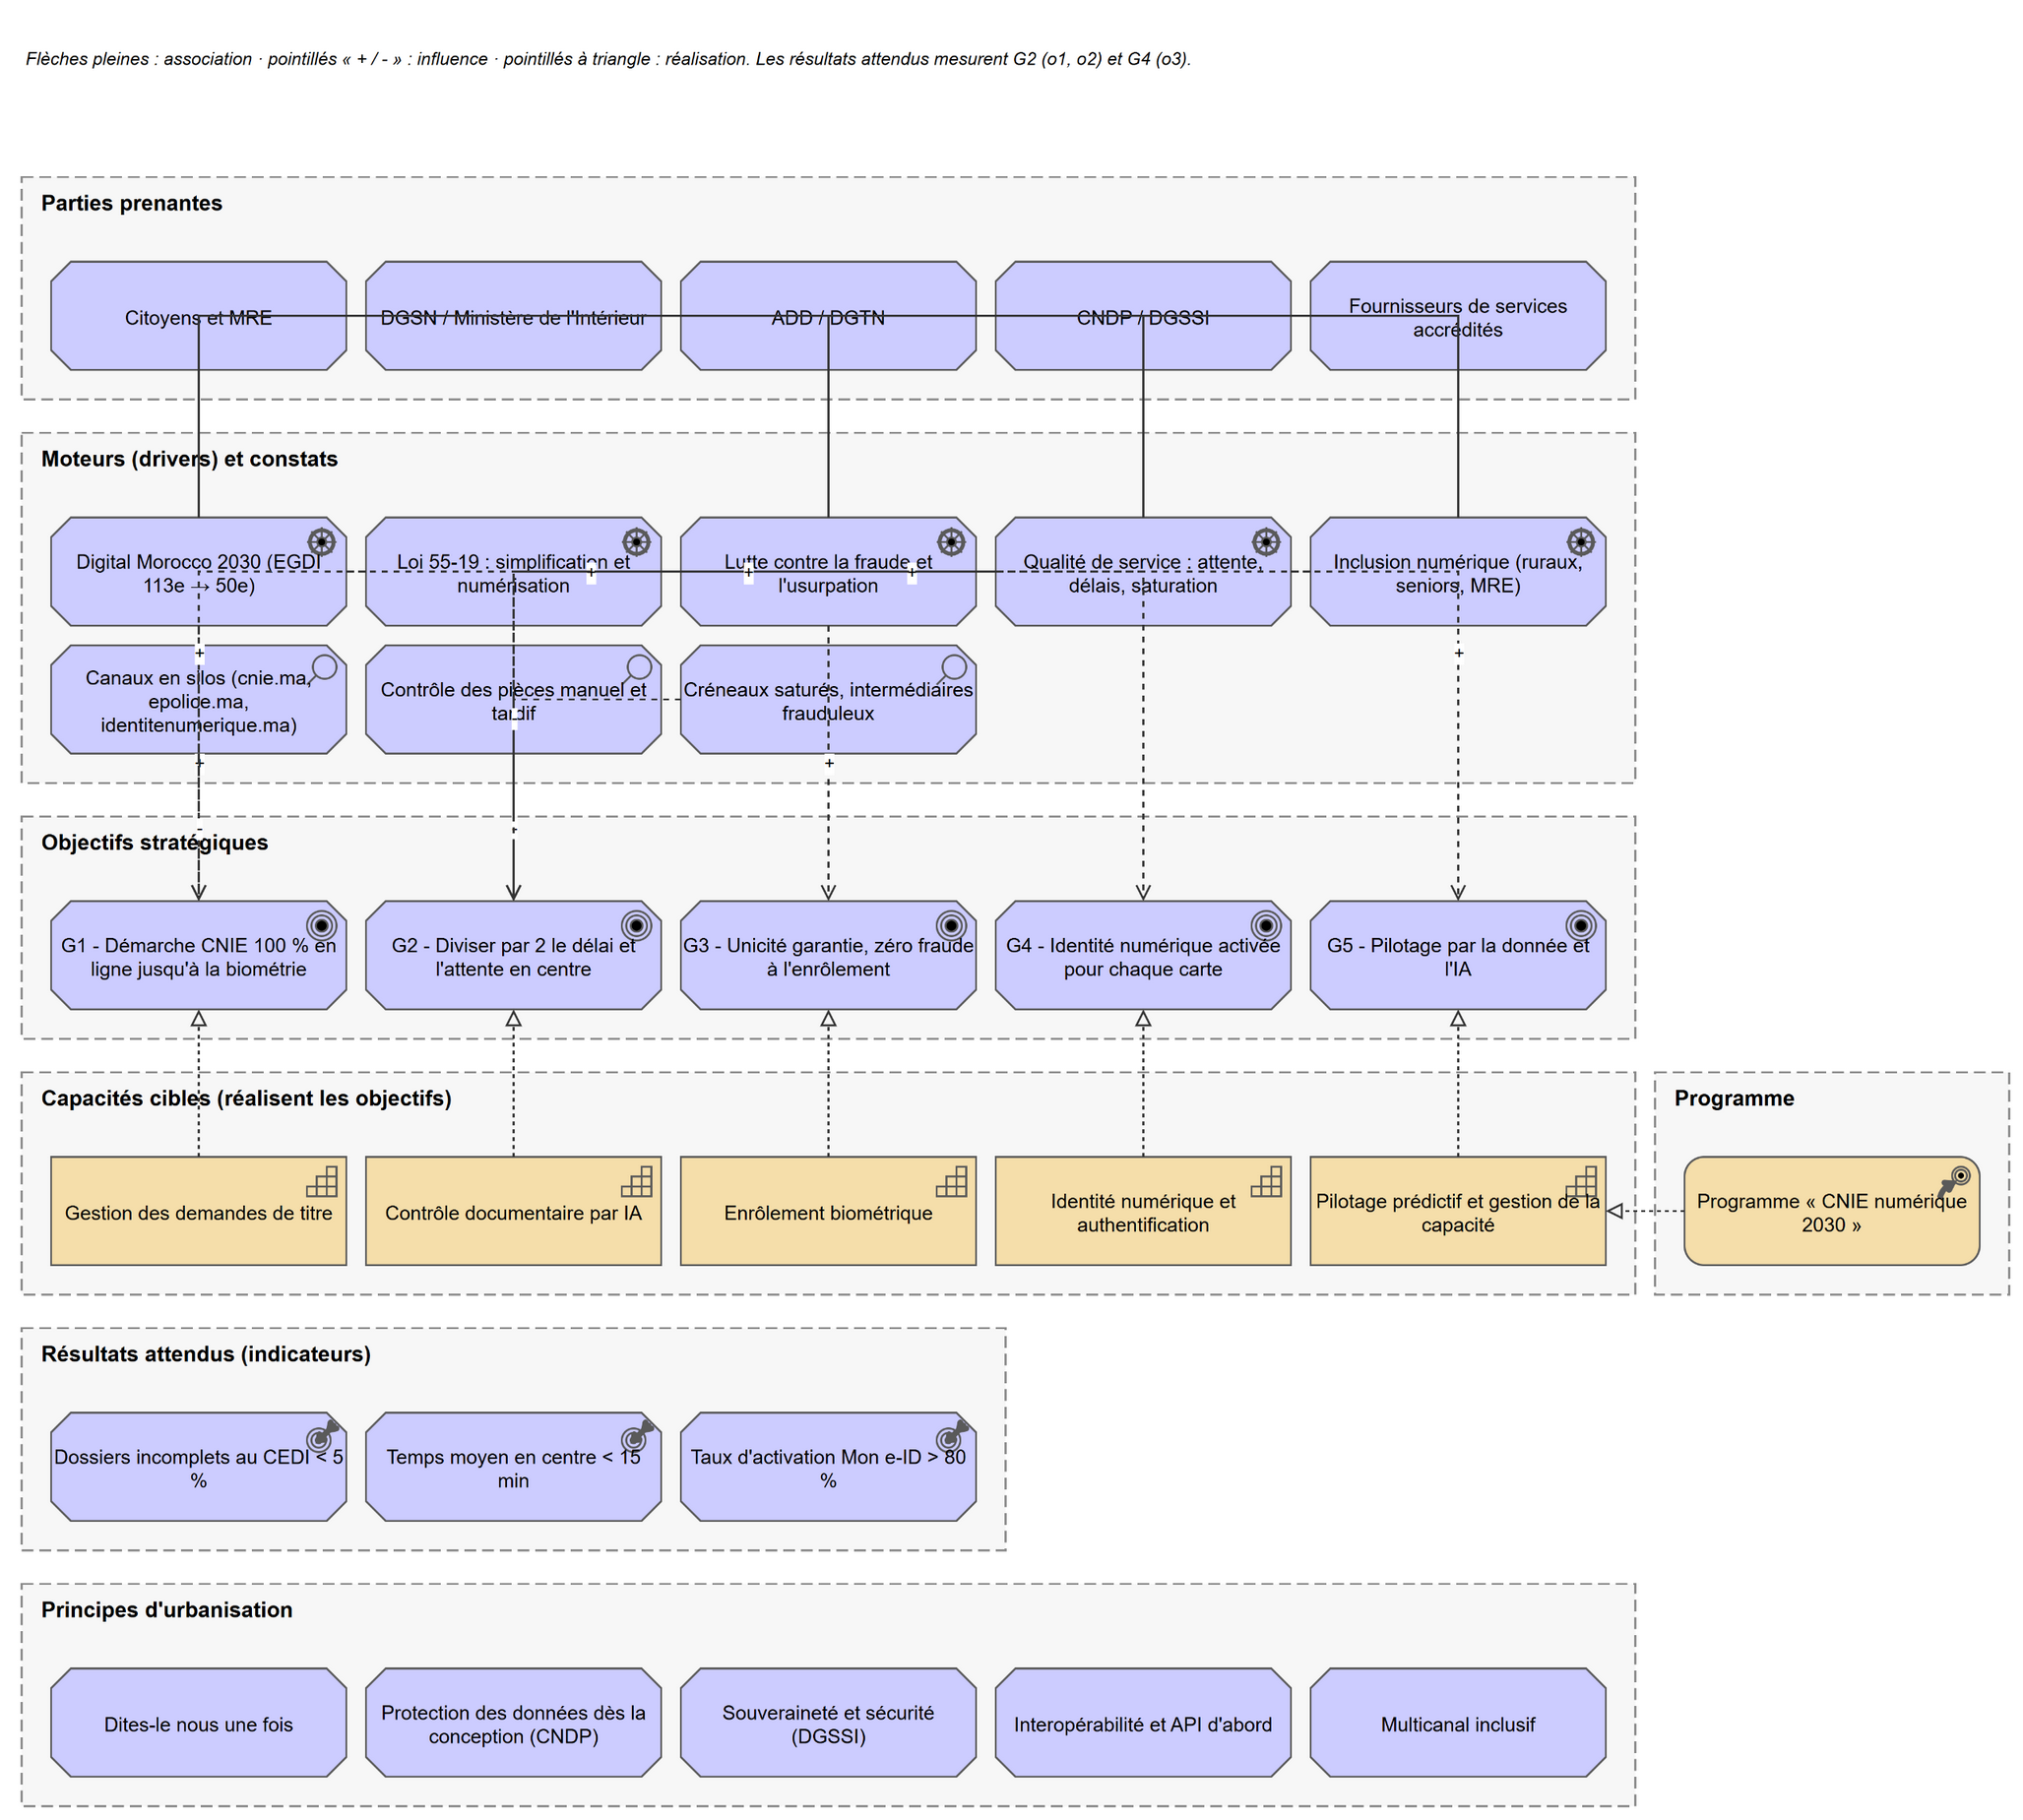
\includegraphics[width=0.95\textwidth]{archimate/V1_motivation.png}
\caption{Vue de motivation et de stratégie~: parties prenantes, moteurs, objectifs, principes et capacités cibles (ArchiMate).}
\label{fig:motivation}
\end{figure*}

\subsection{Principes d'urbanisation}
Cinq principes guident toutes les décisions d'architecture du présent rapport~:
\begin{enumerate}
  \item \textbf{Dites-le nous une fois}~: toute donnée connue de l'État (état civil, adresse, biométrie de référence) est réutilisée après consentement plutôt que redemandée.
  \item \textbf{Protection des données dès la conception}~: minimisation, consentement explicite, séparation des données d'usage et d'identification conformément aux recommandations de la CNDP \cite{cndp_0908}, et maintien du modèle «~les données sont sur la carte~» de la plateforme Tiers de Confiance.
  \item \textbf{Souveraineté et sécurité}~: hébergement national, cryptographie sous HSM, conformité DGSSI, aucune dépendance à un service d'IA hébergé hors du territoire pour les données biométriques.
  \item \textbf{Interopérabilité et API d'abord}~: chaque capacité est exposée par une interface documentée derrière une passerelle unique, ce qui permet d'intégrer les partenaires et de remplacer un composant sans toucher aux autres.
  \item \textbf{Multicanal inclusif}~: le canal numérique devient le canal principal, mais le guichet, l'assistance à domicile et l'assistant conversationnel en arabe, en français et en amazighe garantissent l'accès de tous.
\end{enumerate}

\subsection{Cas d'usage d'intelligence artificielle retenus}
L'intégration de l'IA n'est pas une fin en soi~: chaque cas d'usage répond à un objectif et s'insère à un point précis du processus (tableau~\ref{tab:ia}). Les modèles traitant des données biométriques sont soumis à une évaluation des biais démographiques avant mise en service, les écarts de performance entre groupes de population étant documentés dans la littérature \cite{grother2019frvt}.

\begin{table}[h]
\caption{Cas d'usage d'IA et ancrage dans le processus}
\label{tab:ia}
\centering
\small
\begin{tabularx}{\columnwidth}{lXl}
\toprule
\textbf{Code} & \textbf{Cas d'usage (technique)} & \textbf{Objectif} \\
\midrule
IA-1 & Assistant conversationnel multilingue guidant la saisie (modèle de langue avec recherche documentaire sur la base de connaissances DGSN) & G1, G2 \\
IA-2 & Contrôle documentaire automatique des pièces téléversées~: reconnaissance de caractères, cohérence avec la saisie, conformité de la photo aux critères ICAO \cite{icao9303} & G2 \\
IA-3 & Vérification biométrique à l'enrôlement~: dédoublonnage facial, détection du vivant, rapprochement avec la biométrie de référence & G3 \\
IA-4 & Prévision d'affluence par centre et recommandation de créneaux & G2, G5 \\
IA-5 & Détection d'anomalies sur les demandes et pilotage prédictif des délais & G3, G5 \\
\bottomrule
\end{tabularx}
\end{table}

\subsection{Capacités cibles}
Les objectifs sont réalisés par cinq capacités métier portées par le programme «~CNIE numérique 2030~»~: gestion des demandes de titre, enrôlement biométrique, identité numérique et authentification, contrôle documentaire par IA, pilotage prédictif et gestion de la capacité. Ces capacités constituent la charnière entre la stratégie et les cartographies qui suivent~: chaque bloc fonctionnel et chaque application de la cible contribue à au moins l'une d'elles.
